\documentclass{vkr}
\usepackage[english, russian]{babel} % переносы
\usepackage{graphicx} % для вставки картинок
\graphicspath{{images/}} % путь к изображениям
\usepackage[hidelinks]{hyperref}
\usepackage{float} % определяет метод H для рисунка с переносом на следующую страницу, ели не помещается
\usepackage{pdflscape}
\addto{\captionsrussian}{\renewcommand{\refname}{СПИСОК ИСПОЛЬЗОВАННЫХ ИСТОЧНИКОВ}}
\usepackage{xltabular} % для вставки таблиц
\usepackage{makecell}
\renewcommand\theadfont{} % шрифт в /thead
\usepackage{array} % для определения новых типов столбцов таблиц
\newcolumntype{T}{>{\centering\arraybackslash}X} % новый тип столбца T - автоматическая ширина столбца с выравниванием по центру
\newcolumntype{R}{>{\raggedleft\arraybackslash}X} % новый тип столбца R - автоматическая ширина столбца с выравниванием по правому краю
\newcolumntype{C}[1]{>{\centering\let\newline\\\arraybackslash\hspace{0pt}}m{#1}} % новый тип столбца C - фиксированная ширина столбца с выравниванием по центру
\newcolumntype{r}[1]{>{\raggedleft\arraybackslash}p{#1}} % новый тип столбца r - фиксированная ширина столбца с выравниванием по правому краю
\newcommand{\centrow}{\centering\arraybackslash} % командой \centrow можно центрировать одну ячейку (заголовок) в столбце типа X или p, оставив в оcтальных ячейках другой тип выравнивания
\newcommand{\finishhead}{\endhead\hline\endlastfoot}
\newcommand{\continuecaption}[1]{\captionsetup{labelformat=empty} \caption[]{#1}\\ \hline }
\usepackage{etoolbox}
\AtBeginEnvironment{xltabular}{\refstepcounter{tablecnt}} % подсчет таблиц xltabular, обычные таблицы подсчитываются в классе

\usepackage[tableposition=top]{caption} % подпись таблицы вверху
\captionsetup{strut=off}
\setlength{\intextsep}{0pt} % Vertical space above & below [h] floats
\setlength{\textfloatsep}{0pt} % Vertical space below (above) [t] ([b]) floats
\DeclareCaptionLabelFormat{gostfigure}{Рисунок #2} %подпись рисунка
\DeclareCaptionLabelFormat{gosttable}{Таблица #2} %подпись таблицы
\DeclareCaptionLabelSeparator{gost}{~--~} %разделитель в рисунках и таблицах
\captionsetup{labelsep=gost}
\captionsetup[figure]{aboveskip=10pt,belowskip=4mm,justification=centering,labelformat=gostfigure} % настройка подписи рисунка
\captionsetup[table]{font={stretch=1.41},skip=0pt,belowskip=0pt,aboveskip=8.5pt,singlelinecheck=off,labelformat=gosttable} % настройка подписи таблицы

\setlength{\LTpre}{8mm} % отступ сверху таблицы
\setlength{\LTpost}{6mm} % отступ снизу таблицы

\usepackage{enumitem}
\setlist{nolistsep,wide=\parindent,itemindent=*} % отступы вокруг списков, выравнивание с учетом разделителя

\usepackage{color} %% это для отображения цвета в коде
\usepackage{listings} %% листинги кода
\setmonofont[Scale=0.7]{Verdana} % моноширный шрифт для листинга

\definecolor{codegreen}{rgb}{0,0.6,0}
\definecolor{codegray}{rgb}{0.5,0.5,0.5}
\definecolor{codepurple}{rgb}{0.58,0,0.82}

\lstset{ %
	language=C,                 % выбор языка для подсветки (здесь это С)
	numbers=left,               % где поставить нумерацию строк (слева\справа)
	numberstyle=\tiny,           % размер шрифта для номеров строк
	stepnumber=1,                   % размер шага между двумя номерами строк
	numbersep=5pt,                % как далеко отстоят номера строк от подсвечиваемого кода
	commentstyle=\color{codegreen},
	keywordstyle=\color{magenta},
	numberstyle=\tiny\color{codegray},
	stringstyle=\color{codepurple},
	basicstyle=\linespread{0.95}\ttfamily,
	backgroundcolor=\color{white}, % цвет фона подсветки - используем \usepackage{color}
	showspaces=false,            % показывать или нет пробелы специальными отступами
	showstringspaces=false,      % показывать или нет пробелы в строках
	showtabs=false,             % показывать или нет табуляцию в строках
	frame=single,              % рисовать рамку вокруг кода
	tabsize=2,                 % размер табуляции по умолчанию равен 2 пробелам
	captionpos=t,              % позиция заголовка вверху [t] или внизу [b] 
	breaklines=true,           % автоматически переносить строки (да\нет)
	breakatwhitespace=false, % переносить строки только если есть пробел
	escapeinside={\%*}{*)}   % если нужно добавить комментарии в коде
}

\makeatletter % чтобы допускались русские комментарии в листингах
\lst@InputCatcodes
\def\lst@DefEC{%
	\lst@CCECUse \lst@ProcessLetter
	^^80^^81^^82^^83^^84^^85^^86^^87^^88^^89^^8a^^8b^^8c^^8d^^8e^^8f%
	^^90^^91^^92^^93^^94^^95^^96^^97^^98^^99^^9a^^9b^^9c^^9d^^9e^^9f%
	^^a0^^a1^^a2^^a3^^a4^^a5^^a6^^a7^^a8^^a9^^aa^^ab^^ac^^ad^^ae^^af%
	^^b0^^b1^^b2^^b3^^b4^^b5^^b6^^b7^^b8^^b9^^ba^^bb^^bc^^bd^^be^^bf%
	^^c0^^c1^^c2^^c3^^c4^^c5^^c6^^c7^^c8^^c9^^ca^^cb^^cc^^cd^^ce^^cf%
	^^d0^^d1^^d2^^d3^^d4^^d5^^d6^^d7^^d8^^d9^^da^^db^^dc^^dd^^de^^df%
	^^e0^^e1^^e2^^e3^^e4^^e5^^e6^^e7^^e8^^e9^^ea^^eb^^ec^^ed^^ee^^ef%
	^^f0^^f1^^f2^^f3^^f4^^f5^^f6^^f7^^f8^^f9^^fa^^fb^^fc^^fd^^fe^^ff%
	^^^^20ac^^^^0153^^^^0152%
	% Basic Cyrillic alphabet coverage
	^^^^0410^^^^0411^^^^0412^^^^0413^^^^0414^^^^0415^^^^0416^^^^0417%
	^^^^0418^^^^0419^^^^041a^^^^041b^^^^041c^^^^041d^^^^041e^^^^041f%
	^^^^0420^^^^0421^^^^0422^^^^0423^^^^0424^^^^0425^^^^0426^^^^0427%
	^^^^0428^^^^0429^^^^042a^^^^042b^^^^042c^^^^042d^^^^042e^^^^042f%
	^^^^0430^^^^0431^^^^0432^^^^0433^^^^0434^^^^0435^^^^0436^^^^0437%
	^^^^0438^^^^0439^^^^043a^^^^043b^^^^043c^^^^043d^^^^043e^^^^043f%
	^^^^0440^^^^0441^^^^0442^^^^0443^^^^0444^^^^0445^^^^0446^^^^0447%
	^^^^0448^^^^0449^^^^044a^^^^044b^^^^044c^^^^044d^^^^044e^^^^044f%
	^^^^0401^^^^0451%
	%%%
	^^00}
\lst@RestoreCatcodes
\makeatother

% Режим шаблона (должен быть включен один из трех)
%\ВКРtrue
\Практикаtrue
%\Курсоваяtrue

\newcommand{\Дисциплина}{<<Проектирование и архитектура программных систем>>} % для курсовой
\newcommand{\КодСпециальности}{09.03.04} % Курсовая
\newcommand{\Специальность}{Программная инженерия} % Курсовая
\newcommand{\Тема}{Система управления содержимым веб-сайтов} % ВКР Курсовая
\newcommand{\ТемаВтораяСтрока}{}
\newcommand{\ГдеПроводитсяПрактика}{ООО <<Предприятие ВТИ-Сервис>>} % для практики
\newcommand{\РуководительПрактПредпр}{Куркина А. В.} % для практики
\newcommand{\ДолжнРуководительПрактПредпр}{директор} % для практики
\newcommand{\РуководительПрактУнивер}{Чаплыгин А. А.} % для практики
\newcommand{\ДолжнРуководительПрактУнивер}{к.т.н. доцент} % для практики
\newcommand{\Автор}{Д. И. Украинцев}
\newcommand{\АвторРод}{Украицнва Д.И.}
\newcommand{\АвторПолностьюРод}{Украинцева Дмитрия Игоревича} % для практики
\newcommand{\Шифр}{хх-хх-хххх}
\newcommand{\Курс}{4 } % для практики
\newcommand{\Группа}{ПО-01б}
\newcommand{\Руководитель}{А. А. Чаплыгин} % для ВКР и курсовой
\newcommand{\Нормоконтроль}{А. А. Чаплыгин} % для ВКР
\newcommand{\ЗавКаф}{А. В. Малышев} % для ВКР
\newcommand{\ДатаПриказа}{«07» апреля 2023~г.} % для ВКР
\newcommand{\НомерПриказа}{1505-с} % для ВКР
\newcommand{\СрокПредоставления}{«13» июня 2023~г.} % для ВКР, курсового

\begin{document}
\maketitle
\ifПрактика{}\else{
   \newpage
\begin{center}
\large\textbf{Минобрнауки России}

\large\textbf{Юго-Западный государственный университет}
\vskip 1em
\normalsize{Кафедра программной инженерии}
\vskip 1em
\ifВКР{
        \begin{flushright}
        \begin{tabular}{p{.4\textwidth}}
        \centrow УТВЕРЖДАЮ: \\
        \centrow Заведующий кафедрой \\
        \hrulefill \\
        \setarstrut{\footnotesize}
        \centrow\footnotesize{(подпись, инициалы, фамилия)}\\
        \restorearstrut
        «\underline{\hspace{1cm}}»
        \underline{\hspace{3cm}}
        20\underline{\hspace{1cm}} г.\\
        \end{tabular}
        \end{flushright}
        }\fi
\end{center}
\vspace{1em}
  \begin{center}
  \large
\ifВКР{
ЗАДАНИЕ НА ВЫПУСКНУЮ КВАЛИФИКАЦИОННУЮ РАБОТУ
  ПО ПРОГРАММЕ БАКАЛАВРИАТА}
  \else
ЗАДАНИЕ НА КУРСОВУЮ РАБОТУ (ПРОЕКТ)
\fi
\normalsize
  \end{center}
\vspace{1em}
{\parindent0pt
  Студента \АвторРод, шифр\ \Шифр, группа \Группа
  
1. Тема «\Тема\ \ТемаВтораяСтрока»
\ifВКР{
утверждена приказом ректора ЮЗГУ от \ДатаПриказа\ № \НомерПриказа
}\fi.

2. Срок предоставления работы к защите \СрокПредоставления

3. Исходные данные для создания программной системы:

3.1. Перечень решаемых задач:}

\renewcommand\labelenumi{\theenumi)}

\begin{enumerate}
\item проанализировать IT-инфраструктуру предприятия;
\item  разработать концептуальную модель системы управления IT-ин\-фра\-струк\-турой предприятия на основе подхода к управлению и организации ИТ-услуг ITSM;
\item спроектировать программную систему управления IT-ин\-фра\-струк\-турой предприятия;
\item сконструировать и протестировать программную систему управления IT-инфраструктурой предприятия.
\end{enumerate}

{\parindent0pt
  3.2. Входные данные и требуемые результаты для программы:}

\begin{enumerate}
\item Входными данными для программной системы являются: данные
справочников комплектующих, конфигураций, ПО, критериев качества SLA,
ИТ-услуг, департаментов компании; технические данные ИТ-ресурсов; данные входящих заявок на ИТ-ресурсы; данные запросов поставщикам на комплектующие.
\item Выходными данными для программной системы являются: сформированные заявки на обслуживание ИТ-ресурсов; сформированные запросы на
закупку комплектующих; сведения о выполненных работах по заявкам; статусы заявок; выходные отчеты (инфографика) – по качеству услуг, по состоянию ИТ-ресурсов, по деятельности ИТ-отдела, по стоимости обслуживания
ИТ-ресурсов, воронка заявок.
\end{enumerate}

{\parindent0pt

  4. Содержание работы (по разделам):
  
  4.1. Введение
  
  4.1. Анализ предметной области
  
4.2. Техническое задание: основание для разработки, назначение разработки,
требования к программной системе, требования к оформлению документации.

4.3. Технический проект: общие сведения о программной системе, проект
данных программной системы, проектирование архитектуры программной системы, проектирование пользовательского интерфейса программной системы.

4.4. Рабочий проект: спецификация компонентов и классов программной системы, тестирование программной системы, сборка компонентов программной системы.

4.5. Заключение

4.6. Список использованных источников

5. Перечень графического материала:

\списокПлакатов

\vskip 2em
\begin{tabular}{p{6.8cm}C{3.8cm}C{4.8cm}}
Руководитель \ifВКР{ВКР}\else работы (проекта) \fi & \lhrulefill{\fill} & \fillcenter\Руководитель\\
\setarstrut{\footnotesize}
& \footnotesize{(подпись, дата)} & \footnotesize{(инициалы, фамилия)}\\
\restorearstrut
Задание принял к исполнению & \lhrulefill{\fill} & \fillcenter\Автор\\
\setarstrut{\footnotesize}
& \footnotesize{(подпись, дата)} & \footnotesize{(инициалы, фамилия)}\\
\restorearstrut
\end{tabular}
}

\renewcommand\labelenumi{\theenumi.}

   \abstract{РЕФЕРАТ}

Объем работы равен \formbytotal{lastpage}{страниц}{е}{ам}{ам}. Работа содержит \formbytotal{figurecnt}{иллюстраци}{ю}{и}{й}, \formbytotal{tablecnt}{таблиц}{у}{ы}{}, \arabic{bibcount} библиографических источников и \formbytotal{числоПлакатов}{лист}{}{а}{ов} графического материала. Количество приложений – 2. Графический материал представлен в приложении А. Фрагменты исходного кода представлены в приложении Б.

Перечень ключевых слов: коммерческий сайт, Система, CMS, Битрикс, Joomla, аддитивные технологии, 3D-принтеры, услуги, сервисы, информатизация, автоматизация, информационные технологии, веб-форма,  Apache, классы, база данных, средства защиты информации, подсистема, компонент, модуль, сущность, информационный блок, метод, контент-редактор, администратор, пользователь, web-сайт.

Объектом разработки является web-сайт компании,  занимающейся производством 3D-принтеров, выпуском оборудования для создания порошков, разработкой программного обеспечения и организацией центров аддитивного производства.

Целью выпускной квалификационной работы является привлечение клиентов, увеличение заказов, информирование о продукции и услугах путем создания сайта компании.

В процессе создания сайта были выделены основные сущности путем создания информационных блоков, использованы классы и методы модулей, обеспечивающие работу с сущностями предметной области, а также корректную работу web-сайта, разработаны разделы, содержащие информацию о компании, ее деятельности, производимой продукции и услугах, разработан сервис по заказу 3D-деталей.

При разработке сайта использовалась система управления контентом "<1С-Битрикс: Управление сайтом">.

Разработанный сайт был успешно внедрен в компании.

\selectlanguage{english}
\abstract{ABSTRACT}
  
The volume of work is \formbytotal{lastpage}{page}{}{s}{s}. The work contains \formbytotal{figurecnt}{illustration}{}{s}{s}, \formbytotal{tablecnt}{table}{}{s}{s}, \arabic{bibcount} bibliographic sources and \formbytotal{числоПлакатов}{sheet}{}{s}{s} of graphic material. The number of applications is 2. The graphic material is presented in annex A. The layout of the site, including the connection of components, is presented in annex B.

List of keywords: commercial website, System, CMS, Bitrix, Joomla, additive technologies, 3D printers, services, services, informatization, automation, information technology, web form, Apache, classes, database, component, module, entity, information block, method, content editor, administrator, user, web site.

The object of the research is the analysis of information technologies for the development of a production company's website.

The object of the development is the website of a company engaged in the production of 3D printers, the production of equipment for the creation of powders, software development and the organization of additive manufacturing centers.

The purpose of the final qualifying work is to attract customers, increase orders, inform about products and services by creating a company website.

In the process of creating the site, the main entities were identified by creating information blocks, classes and methods of modules were used to ensure work with the entities of the subject area, as well as the correct operation of the website, sections containing information about the company, its activities, products and services were developed, a service for ordering 3D parts was developed.

When developing the site, the content management system <<1C – Bitrix: Site Management>> was used.

The developed website was successfully implemented in the company.
\selectlanguage{russian}
}\fi
\tableofcontents
\section*{ОБОЗНАЧЕНИЯ И СОКРАЩЕНИЯ}

БД -- база данных.

ИС -- информационная система.

ИТ -- информационные технологии. 

КТС -- комплекс технических средств.

ОМТС -- отдел материально-технического снабжения. 

ПО -- программное обеспечение.

РП -- рабочий проект.

СУБД -- система управления базами данных.

ТЗ -- техническое задание.

ТП -- технический проект.

UML (Unified Modelling Language) -- язык графического описания для объектного моделирования в области разработки программного обеспечения.

\ifПрактика{}\else{\section*{ВВЕДЕНИЕ}
\addcontentsline{toc}{section}{ВВЕДЕНИЕ}

Аддитивные технологии (АТ) начали активно развиваться со времени получения первых трехмерных изображений изделий на дисплеях компьютеров. Начало положила стереолитография, затем довольно многочисленные новые принципы стали называть технологиями быстрого прототипирования, затем укоренилось название "<Аддитивные технологии">. Интенсивность развития данных технологий не имеет аналогов. АТ изменили процессы проектирования и конструирования изделий, превратив их в процессы непрерывного создания изделий. Современные проектирование и производство изделий невозможно представить без данного рода технологий. 3D-принтеры стали такими же распространенными, как и персональные компьютеры. С помощью 3D-принтеров получают ткани, обувь, продукты питания, а также выращивают человеческие органы. Во многих отраслях, например, в космической отрасли, альтернативы аддитивным технологиям нет.

АТ предполагают изготовление детали методом послойного нанесения материала, в отличие от традиционных методов формирования детали, за счёт удаления материала из массива заготовки.

При использовании АТ все стадии реализации проекта от идеи до материализации находятся в единой технологической цепи, в которой каждая технологическая операция выполняется в цифровой CAD/CAM/CAE-системе.

Современные компании, видя, как развиваются информационные технологии, пытаются использовать их выгодно для своего бизнеса, поэтому запускают свой web-сайт. С его помощью предприятие может заявить о себе, проинформировать потенциального заказчика об услугах или продуктах, которые предоставляет, а также позволяет пользователям сделать с помощью сайта онлайн-заказ, произвести покупку или оплатить счета.

Сайт считается лицом компании и может существенно повысить ее имидж. Любой пользователь сети Интернет сможет получить необходимую информацию о компании в любой момент, появляется возможность найти контактные телефоны, адрес и e-mail, чтобы связаться с компанией. Сейчас большинство клиентов узнают о ее существовании именно через сайт. Поэтому сайт можно назвать самой лучшей рекламой. 

Главной задачей профессионально построенного сайта является превращение посетителя, зашедшего на сайт, в потенциального клиента.

\emph{Цель настоящей работы} – разработка web-сайта компании для привлечения новой аудитории, увеличения заказов, рекламы продукции и услуг компании. Для достижения поставленной цели необходимо решить \emph{следующие задачи:}
\begin{itemize}
\item провести анализ предметной области;
\item разработать концептуальную модель web-сайта;
\item спроектировать web-сайт;
\item реализовать сайт средствами web-технологий.
\end{itemize}

\emph{Структура и объем работы.} Отчет состоит из введения, 4 разделов основной части, заключения, списка использованных источников, 2 приложений. Текст выпускной квалификационной работы равен \formbytotal{page}{страниц}{е}{ам}{ам}.

\emph{Во введении} сформулирована цель работы, поставлены задачи разработки, описана структура работы, приведено краткое содержание каждого из разделов.

\emph{В первом разделе} на стадии описания технической характеристики предметной области приводится сбор информации о деятельности компании, для которой осуществляется разработка сайта.

\emph{Во втором разделе} на стадии технического задания приводятся требования к разрабатываемому сайту.

\emph{В третьем разделе} на стадии технического проектирования представлены проектные решения для web-сайта.

\emph{В четвертом разделе} приводится список классов и их методов, использованных при разработке сайта, производится тестирование разработанного сайта.

В заключении излагаются основные результаты работы, полученные в ходе разработки.

В приложении А представлен графический материал.
В приложении Б представлены фрагменты исходного кода. 
}\fi
\section{Анализ предметной области}
\subsection{Обзор истории CMS}
Широкая популярность Интернета обусловнена появлением Всемирной паутины в 1991 году. Изначально считалось, что привлекательность дизайна сайтов не столь важна, как предоставляемая ими информация. Это было связанно с ограниченными возможностями компьютерного оборудования. Веб-сайты были статичными и создавались вручную с использованием HTML-разметки.

С ростом мощности персональных компьютеров и появлением таких технологий как JavaScript (1995) и CSS (1996), интернет стал более наглядным и функциональным.

Параллельно развивалось серверное программирование в 90-е годы, появились языки программирования, такие как PHP (1995), Java (1995), технология Active Server Pages (1996), и система управления базами данных MySQL (1994).

В 2005 году появилась технология AJAX, позволяющая обновлять данные без перезагрузки страницы. Быстрое развитие программного обеспечения привело к разделению веб-сайтов на функциональные блоки: контент (MySQL, HTML), дизайн (CSS) и бизнес-логика (PHP, JavaScript).

В конце 90-х годов наблюдался стремительный рост интернет-контента, что побудило предприятия использовать корпоративные веб-сайты, однако их поддержка в основном выполнялась вручную программистами, затрудняя своевременную публикацию контента. Это создало потребность в системах, автоматизирующих и оптимизирующих процессы работы с контентом, таких как системы управления контентом (CMS).

Первые CMS появились в середине 1990-х годов, разрабатывались организациями самостоятельно и ориентировались на нужды конкретных компаний. В период С 1995 по 1997 годы появились системы управления корпоративным контентом, такие как FileNet, StoryBuilder, Intercloth, Documentum, FatWire, FutureTense и Inso.

С начала 2000-х годов происходит активное создание систем управления веб-контентом (WCMS). В это время утвердилось мнение о том, что современный сайт состоит из двух ключевых компонентов – дизайна и контента. Программисты отвечают за дизайн, а профессионалы в предметной области обеспечивают контент. Это способствовало привлечению большого числа участников к созданию сайтов, что привело к увеличению объема и качества информации в Интернете.

Появление CMS с открытым исходным кодом, таких как Mambo, Drupal, WordPress и Joomla, а также коммерческих CMS, таких как NetCat, Shop-Script, Битрикс: Управление сайтом 3.0 и CS-Cart, сделало создание сайтов доступным для широкого круга пользователей.

WCMS формировались вокруг четырех основных функций: создание контента с использованием редакторов WYSIWYG, управление контентом, публикация контента на сайте и презентация данных для улучшения их визуального представления.

Определились различные группы пользователей, включая дизайнеров, администраторов, команду внедрения и авторов контента. 

Уникальность WCMS обусловлена многочисленными шаблонами, плагинами и доступом к CSS.

Тем не менее, первые WCMS имели некоторые недостатки, такие как сложность конфигурации CSS, ограниченную функциональность редакторов WYSIWYG и ограниченный круг пользователей, способных создавать контент.

На дальнейшее развитие WCMS, оказали влияние несколько выжных факторов.

Во-первых, это дальнейшее развитие вычислительной техники. Мощность современных смартфонов превосходит ту, которую имел персональный компьютер 20 лет назад.

Во-вторых, появление в 2005 году концепции и технологии Web 2.0, социальных сетей и облачных вычислений. Web 2.0 расширил возможности Интернета в целом и WCMS в частности. Теперь не только отдельные люди, но и целые сообщества могли вносить свой вклад в информационные ресурсы, что привело к увеличению объема доступной информации. В результате возникла потребность в более простых инструментах для работы с контентом, таких как вики-разметка и онлайн-редакторы. Это также вызвало рост спроса на интерфейсы, ориентированные на непрофессионалов в информационных системах. Появляются новые более удобные и функциональные версии редакторов WYSIWYG, а установка и первоначальная настройка WCMS стала гораздо быстрее и проще. Рост социальных сетей требует интеграции с ними WCMS, которая происходит через плагины для автоматического связывания и регистрации через социальные сети.

Третий фактор -- быстрое развитие мобильных технологий и увеличение трафика с мобильных устройств влияет на тенденции развития веб-сайтов.

\subsection{Основные понятия CMS}
CMS -- программный комплекс, используемый для обеспечения и организации совместного процесса создания, редактирования и контроля содержимого веб-страниц. Содержимое может включать текст, изображения, видео, аудиофайлы, документы, мультимедийные файлы и многое другое.

CMS позволяет нетехническим пользователям легко управлять и обновлять контент на веб-сайте, не требуя навыков программирования или веб-разработки.

CMS, как правило, имеет модульную архитектуру, обеспечивающую легкую интеграцию плагинов и расширений, которые могут быть настроены для удовлетворения конкретных требований или расширения функциональности.

Пользователи CMS, такие как авторы или редакторы, создают контент с помощью  WYSIWYG редактора, позволяющего легко форматировать и манипулировать текстом, изображениями и мультимедийными компонентами.

Созданный контент хранится в базе данных вместе с метаданными, такими как информация об авторе, категории и теги, которые облегчают организацию и возможность поиска.

Авторизованные пользователи могут управлять содержимым, выполняя такие действия, как редактирование, просмотр, утверждение или удаление содержимого, а также управление ролями пользователей и разрешениями на доступ.

Когда пользователь запрашивает определенную страницу или ресурс, CMS извлекает соответствующий контент из базы данных, обрабатывает его, используя шаблоны и темы для стилизации, и генерирует окончательный HTML-документ, который затем передается в веб-браузер пользователя.

\subsection{Структура CMS}
Хотя платформы CMS могут различаться по функциональности, у них есть общие основные компоненты. Эти компоненты включают в себя:
\begin{itemize}
	\item приложение для управления контентом (CMA). Приложение для управления контентом (CMA) -- это пользовательский интерфейс, который позволяет создателям и редакторам контента создавать, изменять и удалять контент с веб-сайта без необходимости наличия технических знаний. Это часть CMS, которую чаще всего используют создатели контента и администраторы;
	\item приложение доставки контента (CDA). Приложение доставки контента (CDA) отвечает за хранение и доставку контента конечным пользователям. Он извлекает содержимое из базы данных, объединяет его с соответствующими шаблонами и отображает на веб-сайте. Этот процесс происходит в фоновом режиме и невидим для создателей контента и администраторов;
	\item база данных. База данных хранит и упорядочивает контент и метаданные веб-сайта. Платформы CMS обычно используют базы данных для хранения контента, шаблонов, пользовательской информации и конфигураций.
\end{itemize}

\subsection{Классификация CMS}
Существует несколько типов CMS, каждая из которых отличается архитектурой, функциональностью и вариантами использования. Выделяют три основных типа CMS:
\begin{itemize}
	\item монолитная (связанная) CMS. Монолитная или совмещенная CMS -- это традиционная система управления контентом с тесно интегрированными уровнями управления контентом и представления. Этот тип CMS поставляется со встроенными шаблонами и инструментами дизайна для создания и поддержания внешнего вида веб-сайта. Монолитные платформы CMS обычно предлагают более оптимизированный опыт для нетехнических пользователей, но они могут быть менее гибкими, чем безголовые или развязанные варианты CMS;
	\item безголовая CMS. Безголовая CMS -- это система управления контентом, которая не имеет внешнего интерфейса или уровня представления. Вместо этого контент отделен от представления, что позволяет разработчикам выбирать любую интерфейсную технологию для отображения контента. В безголовой CMS контент управляется через API (программные интерфейсы приложений), которые могут обслуживать контент на нескольких устройствах и платформах, что делает его популярным выбором для предприятий с несколькими каналами доставки, такими как веб-сайты, мобильные приложения и устройства IoT;
	\item развязанная CMS. Развязанная CMS -- это гибрид безголовой и традиционной монолитной (связанной) CMS. Как и безголовая CMS, несвязанная CMS отделяет управление контентом от уровня представления. Тем не менее, он также включает в себя встроенные интерфейсные шаблоны и инструменты, позволяющие создавать и предварительно просматривать контент перед запуском. Это позволяет создателям контента иметь больший контроль над представлением своего контента, в то же время используя преимущества гибкости и масштабируемости несвязанной архитектуры.
\end{itemize}
\section{Техническое задание}
\subsection{Основание для разработки}

Основанием для разработки является задание на выпускную квалификационную работу бакалавра "<Разработка системы управления содержимым веб-сайтов">.

\subsection{Цель и назначение разработки}

Разрабатываемая программно-информационная система предназначена для совместного создания и управления веб-сайтами, не требуя от пользователей навыков программирования и веб-разработки. 

Задачами данной разработки являются:
\begin{itemize}
	\item разработка пользовательского интерфейса (административной панели) системы;
	\item разработка структуры базы данных для хранения информации о сущностях системы;
	\item разработка серверной части системы;
	\item разработка визуального редактора контента;
	\item реализация управления пользователями и правами доступа;
	\item реализация возможности выбора и применения различных тем (шаблонов) веб-сайта;
	\item реализация возможности совместной работы нескольких пользователей над контентом;
	\item организация хранилища медиафайлов.
\end{itemize}

\subsection{Требования к программной системе}
\subsubsection{Требования к данных программной системы}

Входными данными для программной системы являются:
\begin{itemize}
	\item содержимое страниц и записей (постов): текст, медиафайлы;
	\item категории и теги для организации записей (постов);
	\item метаданные для страниц: заголовок, описание, ключевые слова;
	\item пользовательские данные: регистрационная информация (имя пользователя, пароль);
	\item файлы темы (шаблона) оформления сайта;
	\item настройки и параметры: название, адрес сайта.
\end{itemize}

Выходными данными для программной системы будут:
\begin{itemize}
	\item отображение данных в виде веб-страниц;
	\item вывод содержимого медиафайлов на веб-страницах;
	\item использование тем (шаблонов) для оформления содержимомого страниц сайта;
	\item применение настроек и параметров к сайту.
\end{itemize}

\subsubsection{Функциональные требования к программной системе}

На основании анализа предметной области в разрабатываемой программной системе должны быть реализованы следующие функции:
\begin{enumerate}
	\item Аутентификация и авторизация пользователей.
	\item Управление веб-страницами.
	\item Управление записями (постами).
	\item Управление категориями и тегами записей (постов).
	\item Управление меню и навигацией на сайте.
	\item Управление темой (шаблоном) сайта.
	\item Управление пользователями.
	\item Управление настройками сайта.
\end{enumerate}

На рисунке \ref{usecase:image} представлены функциональные требования к системе в виде диаграммы прецедентов нотации UML.

\begin{figure}[ht]
	\center{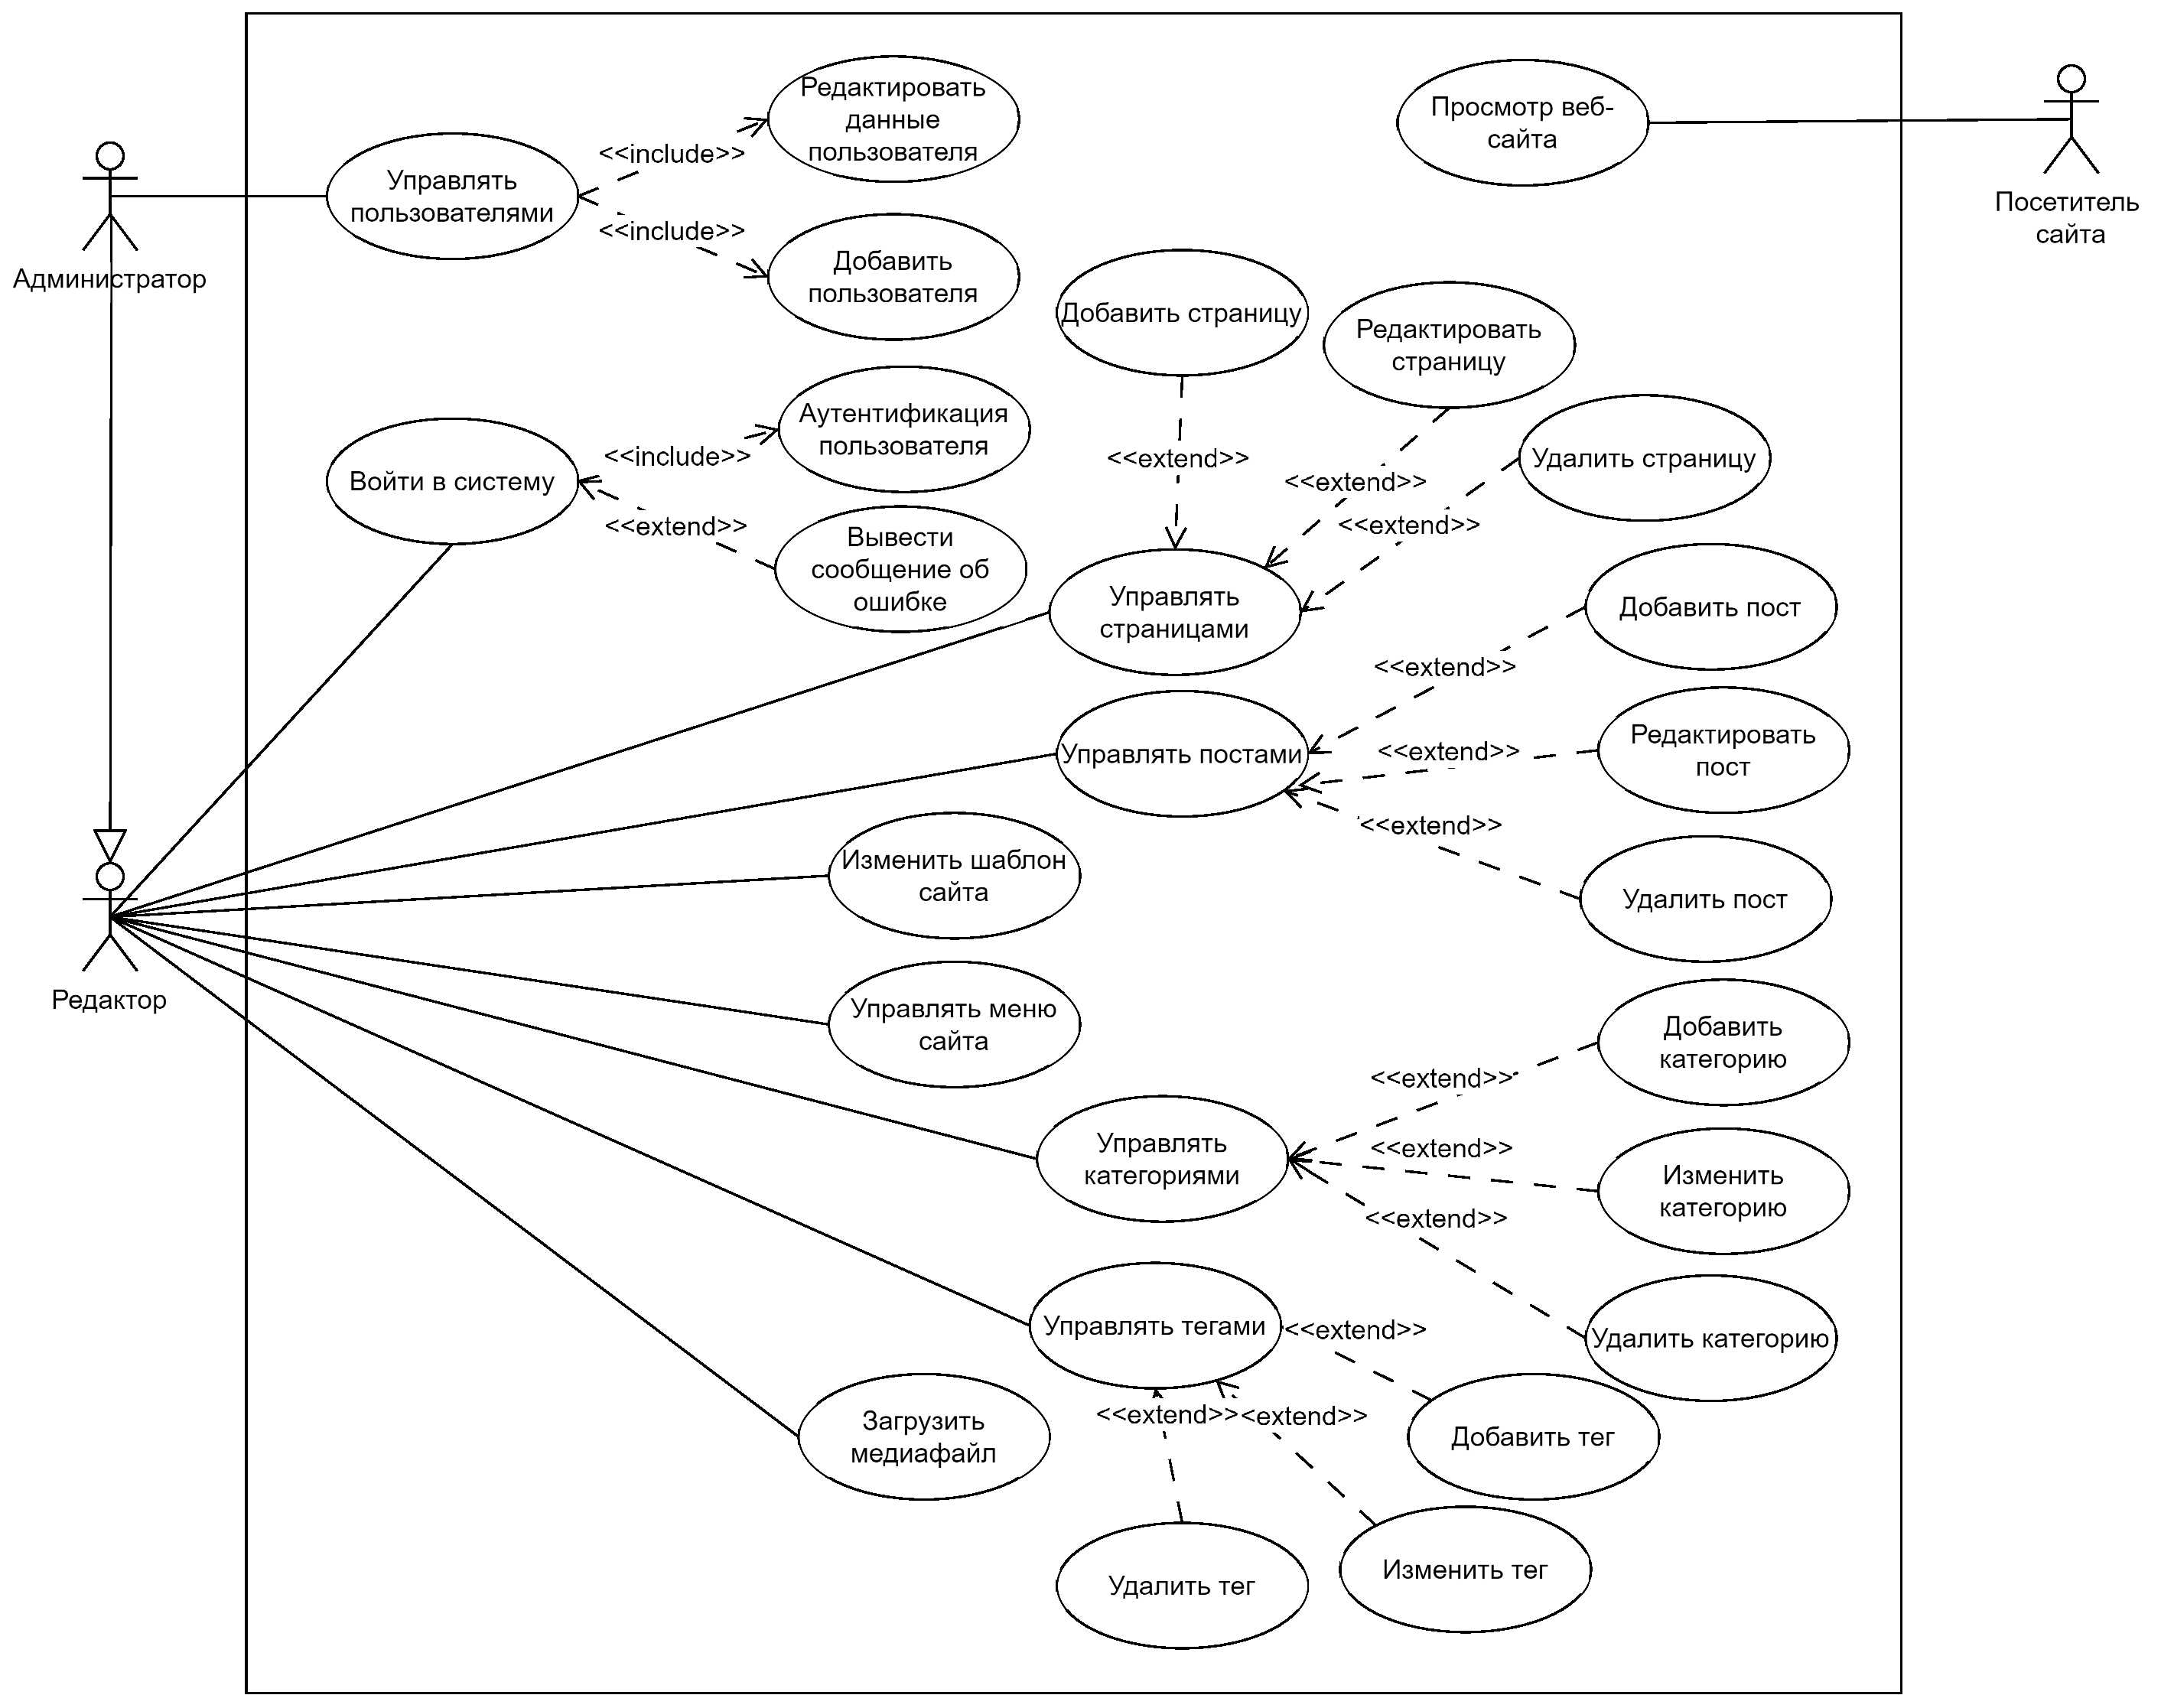
\includegraphics[width=1\linewidth]{usecase}}
	\caption{Диаграмма прецедентов}
	\label{usecase:image}
\end{figure}

\subsubsection{Моделирование вариантов использования}
\paragraph{Вариант использования <<Войти в систему>>}
Заинтересованные лица и их требования: пользователь хочет поулчить доступ к административной панели сайта.

Предусловие: пользователь зарегистрирован в системе и знает свои данные для входа (логин и пароль).

Постусловие: система авторизует пользователя в соответствии с его ролью.

Основной успешный сценарий:
\begin{enumerate}
	\item Пользователь вводит адрес административной панели сайта в браузере для перехода на страницу входа в систему.
	\item Пользователь вводит логин и пароль.
	\item Система проверяет корректность введенных данных и аутентифицирует пользователя.
	\item Пользователь перенаправляется на главную страницу административной панели сайта.
\end{enumerate}

\paragraph{Вариант использования <<Управлять пользователями>>}
Заинтересованные лица и их требования: администратор хочет управлять учетными записями пользователей и их ролями в системе.

Предусловие: пользователь авторизован и имеет права администратора.

Постусловие: изменения в учетных записях пользователей сохранены в системе.

Основной успешный сценарий:
\begin{enumerate}
	\item Администратор открывает раздел управления пользователями.
	\item Администратор выбирает действие (создание, редактирование, удаление пользователя).
	\item Администратор вводит необходимую информацию о пользователе.
	\item Система сохраняет изменения и обновляет список пользователей.
\end{enumerate}

\paragraph{Вариант использования <<Управлять страницами сайта>>}
Заинтересованные лица и их требования: пользователь хочет управлять страницами сайта.

Предусловие: пользователь авторизован в системе и имеет соответствующие права доступа.

Постусловие: изменения сохранены и отображаются на сайте.

Основной успешный сценарий:
\begin{enumerate}
	\item Пользователь открывает раздел управления страницами.
	\item Пользователь создает новую страницу или выбирает существующую для редактирования.
	\item Пользователь переходит в режим редактирования страницы.
	\item Пользователь добавляет новый или выбирает существующуй элемент страницы для редактирования.
	\item Пользователь вносит необходимые изменения в содержимое элемента.
	\item Пользователь вносит необходимую информацию о странице (название, URL, метаданные).
	\item Пользователь сохраняет изменения.
\end{enumerate}

\paragraph{Вариант использования <<Управлять постами>>}
Заинтересованные лица и их требования: пользователь хочет упралять постами.

Предусловие: пользователь авторизован в системе и имеет соответствующие права доступа.

Постусловие: изменения в постах сохранены и отображаются на соответствующей странице сайта.

Основной успешный сценарий:
\begin{enumerate}
	\item Пользователь открывает раздел управления постами.
	\item Пользователь создает новый пост или выбирает существующий для редактирования.
	\item Пользователь вносит необходимые изменения в текст, заголовок, метаданные и т. д..
	\item Пользователь сохраняет или публикует новый пост.
\end{enumerate}

\paragraph{Вариант использования <<Управлять категориями и тегами постов>>}
Заинтересованные лица и их требования: пользователь хочет управялть категориями и тегами постов.

Предусловие: пользователь авторизован в системе и имеет соответствующие права доступа.

Постусловие: изменения в категориях и тегах сохранены и применены к соответствующим постам.

Основной успешный сценарий:
\begin{enumerate}
	\item Пользователь открывает подраздел управления категориями и тегами постов.
	\item Пользователь создает новую категорию/тег или редактирует существующие.
	\item Пользователь присваивает их соответствующим постам.
	\item Система сохраняет изменения и реорганизует отображение постов.
\end{enumerate}

\paragraph{Вариант использования <<Управлять меню и навигацией сайта>>}
Заинтересованные лица и их требования: пользователь хочет управялть навигационным меню сайта.

Предусловие: пользователь авторизован в системе и имеет соответствующие права доступа.

Постусловие: изменения в меню сохранены и отображаются на сайте.

Основной успешный сценарий:
\begin{enumerate}
	\item Пользователь открывает раздел управления меню и навигацией сайта.
	\item Пользователь создает новый пункт меню, редактирует существующие.
	\item Пользователь изменяет их порядок или структуру.
	\item Пользователь сохраняет изменения.
\end{enumerate}

\paragraph{Вариант использования <<Изменить шаблон>>}
Заинтересованные лица и их требования: пользователь хочет изменить шаблон дизайна сайта.

Предусловие: пользователь авторизован в системе и имеет соответствующие права доступа.

Постусловие: выбранный шаблон применен к страницам сайта.

Основной успешный сценарий:
\begin{enumerate}
	\item Пользователь открывает раздел управления шаблонами административной панели.
	\item Пользователь выбирает одну из доступных тем (шаблонов).
	\item Пользователь нажимает соответствующую кнопку для активации темы (шаблона).
	\item Система сохраняет изменения и обновляет шаблон сайта.
\end{enumerate}

\paragraph{Вариант использования <<Загрузить медиафайл>>}
Заинтересованные лица и их требования: пользователь хочет иметь возможность загрузки и удаления медиафайлов.

Предусловие: пользователь авторизован в системе и имеет соответствующие права доступа.

Постусловие: медиафайлы загружены и доступны для использования на сайте.

Основной успешный сценарий:
\begin{enumerate}
	\item Пользователь открывает раздел управления медиафайлами административной панели.
	\item Пользователь нажимает соответствующую кнопку для загрузки файла и выбирает файл.
	\item Система сохраняет файл в соответствующую папку на сервере.
\end{enumerate}

\subsubsection{Требования пользователя к интерфесу программной системы} \label{interface_requirements}
Интрефейс пользователя административной панели разрабатываемой системы управления содержимым должен включать следующие компоненты:
\begin{enumerate}
	\item Навигационное меню.
	\item Редактор контента.
	\item Интерфейс управления страницами сайта.
	\item Интерфейс управления записями (постами).
	\item Интерфейс управления виджетами.
	\item Интерфейс управления меню и навигацией на сайте.
	\item Интерфейс управления пользователями.
	\item Интерфейс управления темами (шаблонами) сайта.
	\item Интерфейс управления медиафайлами.
\end{enumerate}

Навигационное меню предназначено для перемещения по разделам и функциям CMS.

Интерфейс редактора контента включает панели инструментов с кнопками для форматирования текста, добавления ссылок, вставки изображений, видео, таблиц и т. д.

Интерфейс управления страницами сайта отображает список страниц сайта, включает кнопки для создания, редактирования, удаления страниц, поля для ввода данных страницы при добавлении или редактировании страницы.

Интерфейс управления записями (постами) отображает список записей, включает кнопки для создания, редактирования, удаления записей, поля для ввода данных при добавлении или редактировании записи.

Интерфейс управления медиафайлами отображает список загруженных файлов и включает кнопки для загрузки, просмотра, редактирования и удаления медиафайлов.

Интерфейс управления пользователями отображает список пользователей системы и включает кнопки для создания, редактирования и удаления учетных записей пользователей.

Интерфейс управления шаблонами отображает список доступных тем (шаблонов) и кнопку для активации выбранной темы.

Интерфейс управления меню и навигацией включает возможность управления навигационными меню и ссылками на страницы.

При реализации пользовательского интерфейса должны быть использованы следующие технологии:
\begin{itemize}
	\item язык разметки веб-страниц HTML -- для описания структуры страниц веб-интерфейса;
	\item каскадные таблицы стилей СSS -- для стилизации элементов интерфейса;
	\item язык программирования JavaScript -- для создания интерактивного интерфейса;
	\item библиотека jQuery языка программирования JavaScript -- для обмена данными с сервером и обновления элементов интерфейса.
\end{itemize}

\subsection{Нефункциональные требования к программной системе}
\subsubsection{Требования к надежности}
В приложении не должно возникать критических ошибок, приводящих к экстренному завершению работы.
\subsubsection{Требования к программному обеспечению}
Для реализации программной системы должены быть использованы следующие технологии:
\begin{itemize}
	\item язык программирования PHP -- для разработки серверной части;
	\item СУБД MySQL -- для хранения данных и организации данных;
	\item веб-сервер Apache HTTP Server -- для обработки клиентских запросов.
\end{itemize}

\subsubsection{Требования к аппаратному обеспечению}
Для работы приложения, установленного на компьютер, необходимо дисковое пространство не менее 100 Мб, свободная оперативная память в размере не менее 1024 Мб, видеокарта с не менее 1024 Мб видеопамяти, клавиатура, мышь, установленная операционная система Windows, macOS или Linux, архитектура процессора х86 (Windows) или x64 (Windows, macOS, Linux). 

Для доступа к административной панели системы, потребуется браузер Google Chrome, Mozilla Firefox или Microsoft Edge.
\subsubsection{Требования к оформлению документации}
Разработка программной документации и программного изделия должна производиться согласно ГОСТ 19.102-77 и ГОСТ 34.601-90. Единая система программной документации.
\section{Технический проект}
\subsection{Общая характеристика организации решения задачи}

Необходимо спроектировать и разработать серверную и клиентскую части программно-информационной системы.

Система управления содержимым веб-сайта состоит из различных компонентов, предназначенных для управления, создания, редактирования и публикации контента на веб-сайте. Основные компоненты разрабатываемой CMS:
\begin{enumerate}
	\item Интерфейс управления (административная панель).
	\item База данных.
	\item Редактор контента.
	\item Шаблоны и темы.
\end{enumerate}

При разработке программы должно быть уделено внимание следующим ключевым аспектам:
\begin{enumerate}
	\item Простота использования.
	\item Масштабируемость.
	\item Безопасность.
	\item Производительность.
\end{enumerate}

\subsection{Обоснование выбора технологии проектирования}

Выбранные для разработки программно-информационной системы языки и технологии предоставляют функции для создания эффективных и функциональных кроссбраузерных веб-приложений, позволяя создавать легко поддерживаемые и масштабируемые программные продукты.

\subsubsection{Описание используемых технологий и языков программирования}


\paragraph{Язык программирования PHP}

%PHP – язык для написания сценариев, исполняемых на компьютере web-приложения посредством интерпретации исходного кода \cite{php}. Основное предназначение данного языка – это выполнение на сервере сценариев, создающих динамические web-страницы.
PHP (Hypertext Preprocessor) -- распространённый интерпретируемый язык общего назначения с открытым исходным кодом, который создавался специально для ведения веб-разработок, и код на нём встраивается непосредственно в HTML-код. Синтаксис языка берёт начало из языков C, Java и Perl и лёгок для изучения. Основная цель языка -- помочь веб-разработчикам создавать динамически генерируемые веб-страницы. 

Главная область применения PHP -- написание скриптов, работающих на стороне сервера; таким образом, PHP способен выполнять все то, что выполняет любая другая программа CGI, например, обрабатывать данные форм, генерировать динамические страницы или отсылать и принимать cookies. 

PHP отличается от JavaScript тем, что PHP-скрипты выполняются на сервере и генерируют HTML, который посылается клиенту. 

Существуют три основных области применения PHP:
\begin{itemize}
	\item cоздание скриптов для выполнения на стороне сервера;
	\item cоздание скриптов для выполнения в командной строке;
	\item cоздание оконных приложений, выполняющихся на стороне клиента.
\end{itemize}

PHP доступен для большинства операционных систем, включая Linux, многие модификации Unix (такие как HP-UX, Solaris и OpenBSD), Microsoft Windows, macOS, RISC OS и многие другие. Также в PHP включена поддержка большинства современных веб-серверов, таких как Apache, IIS и многих других.

Таким образом, PHP предоставляет свободу выбора операционной системы и веб-сервера. Более того, появляется выбор между использованием процедурного или объектно-ориентированного программирования (ООП) или же их сочетания.

Использование PHP не ограничивается выводом HTML. Возможности PHP включают вывод файлов различных типов, таких как изображения или PDF-файлы, шифрование данных и отправку электронной почты. Можно выводить любой текст, например JSON или XML. PHP может автоматически генерировать эти файлы и сохранять их в файловой системе вместо вывода на печать, формируя серверный кеш для динамического содержимого.

Одним из значительных преимуществ PHP является поддержка широкого круга баз данных. Можно воспользоваться модулем, специфичным для отдельной базы данных (таким как mysql) или использовать уровень абстракции от базы данных, такой как PDO, или подсоединиться к любой базе данных, поддерживающей Открытый Стандарт Соединения Баз Данных (ODBC), с помощью одноимённого модуля ODBC.

PHP также поддерживает взаимодействие с другими сервисами через такие протоколы, как LDAP, IMAP, SNMP, NNTP, POP3, HTTP, COM (на платформах Windows) и многих других.

\paragraph{Язык программирования JavaScript}
JavaScript -- это интерпретируемый язык программирования высокого уровня, который в основном используется в качестве языка сценариев для веб-разработки. Это одна из трех основных технологий Всемирной паутины наряду с HTML и CSS.

Язык программирования JavaScript позволяет создавать интерактивные веб-страницы и является неотъемлемой частью веб-приложений. В то время как HTML определяет структуру и макет веб-страницы, а CSS придает ей стиль, JavaScript делает ее интерактивной, обеспечивая динамическое содержание и взаимодействие с пользователем.

Веб-браузеры имеют встроенные механизмы для интерпретации и выполнения скриптов JavaScript, что позволяет языку работать непосредственно в браузере (фронтенд) без компилятора. Эта особенность JavaScript делает его языком клиентской стороны, хотя он также может использоваться на стороне сервера (бэкенд) с помощью таких сред, как Node.js.

Язык JavaScript поддерживает объектно-ориентированное программирование с прототипным наследованием, а также императивный и функциональный стили программирования. В нем есть API для работы с текстом, массивами, датами, регулярными выражениями и объектной моделью документа (DOM), но он не включает никаких средств ввода-вывода, таких как сеть, хранилище или графические средства, полагаясь для этого на среду хоста, в которую он встроен.

\paragraph{Библиотека jQuery}
jQuery -- это быстрая, небольшая и многофункциональная библиотека языка программирования JavaScript, которая предоставляет множество полезных функций и инструментов для создания интерактивных и функциональных веб-приложений.

Одной из основных функций jQuery является возможность манипулировать HTML элементами на странице. С помощью этой библиотеки можно легко добавлять новые элементы, изменять их атрибуты или стили, а также удалять ненужные элементы.

jQuery позволяет легко обрабатывать различные виды событий на веб-странице. Например, можно обрабатывать клики по кнопкам, наведение курсора на элементы и многое другое.

jQuery упрощает использование AJAX-запросов, позволяя разработчикам отправлять асинхронные запросы на сервер без перезагрузки всей страницы.

\paragraph{Технология AJAX}
AJAX (аббревиатура от Asynchronous JavaScript and XML) – это технология взаимодействия с сервером без перезагрузки страницы. Поскольку не требуется каждый раз обновлять страницу целиком, повышается скорость работы с сайтом и удобство его использования.

В работе технологии можно выделить 4 основных этапа:
\begin{enumerate}
	\item Пользователь вызывает AJAX. Обычно это реализуется с помощью какой-либо кнопки, предлагающей получить больше информации.
	\item Система отправляет на сервер запрос и всевозможные данные. Например, может потребоваться загрузка определенного файла либо конкретных сведений из базы данных.
	\item Сервер получает ответ от базы данных и отправляет информацию в браузер.
	\item JavaScript получает ответ, расшифровывает его и выводит пользователю.
\end{enumerate}

Для обмена данными на странице создается объект XMLHttpRequest, он будет выполнять функцию посредника между браузером и сервером. Запросы могут отправляться в одном двух типов – GET и POST. Серверная часть обрабатывает поступающие данные и на их основании создает новую информацию, которая будет отправлена клиенту.

AJAX применяет асинхронную передачу данных. Такой подход позволяет пользователю совершать различные действия во время «фонового» обмена информации с сервером.

В качестве ответа сервер использует простой текст, XML и JSON.

\subsection{Проектирование архитектуры программной системы}
\subsubsection{Описание сущностей программной системы}
Исходя из требований изложенных в технческом задании, можно выделить следующие основные сущности проектируемой системы:
\begin{itemize}
	\item "<Пользователь">;
	\item "<Страница">;
	\item "<Пост">;
	\item "<Категория">;
	\item "<Тег">;
	\item "<Пункт меню">.
\end{itemize}

В состав сущности "<Пользователь"> можно включить атрибуты, представленные в таблице \ref{user:table}.
\begin{xltabular}{\textwidth}{|l|l|p{1.7cm}|X|}
	\caption{Атрибуты сущности "<Пользователь">\label{user:table}}\\ \hline
	\centrow Поле & \centrow Тип & \centrow Обяза\-тельное & \centrow Описание \\ \hline
	\thead{1} & \thead{2} & \centrow 3 & \centrow 4 \\ \hline
	\endfirsthead
	\continuecaption{Продолжение таблицы \ref{user:table}}
	\thead{1} & \thead{2} & \centrow 3 & \centrow 4 \\ \hline
	\finishhead
	\_id & Integer & true & Уникальный идентификатор \\ \hline
	username & String & true & Логин \\ \hline
	name & String & true & Имя пользователя \\ \hline
	password\_hash & String & true & Хэш пароля
\end{xltabular}

В состав сущности "<Страница"> можно включить атрибуты, представленные в таблице \ref{page:table}.
\begin{xltabular}{\textwidth}{|l|l|p{1.7cm}|X|}
	\caption{Атрибуты сущности "<Страница">\label{page:table}}\\ \hline
	\centrow Поле & \centrow Тип & \centrow Обяза\-тельное & \centrow Описание \\ \hline
	\thead{1} & \thead{2} & \centrow 3 & \centrow 4 \\ \hline
	\endfirsthead
	\continuecaption{Продолжение таблицы \ref{page:table}}
	\thead{1} & \thead{2} & \centrow 3 & \centrow 4 \\ \hline
	\finishhead
	\_id & Integer & true & Уникальный идентификатор \\ \hline
	title & String & true & Название страницы \\ \hline
	content & Text & true & Содержимое страницы \\ \hline
	parent\_page\_id & Integer & false & Идентификатор родительской страницы
\end{xltabular}

В состав сущности "<Пост"> можно включить атрибуты, представленные в таблице \ref{post:table}.
\begin{xltabular}{\textwidth}{|l|l|p{1.7cm}|X|}
	\caption{Атрибуты сущности "<Пост">\label{post:table}}\\ \hline
	\centrow Поле & \centrow Тип & \centrow Обяза\-тельное & \centrow Описание \\ \hline
	\thead{1} & \thead{2} & \centrow 3 & \centrow 4 \\ \hline
	\endfirsthead
	\continuecaption{Продолжение таблицы \ref{post:table}}
	\thead{1} & \thead{2} & \centrow 3 & \centrow 4 \\ \hline
	\finishhead
	\_id & Integer & true & Уникальный идентификатор \\ \hline
	title & String & true & Название поста \\ \hline
	content & Text & true & Содержимое поста \\ \hline
	author\_id & Integer & true & Идентификатор автора поста \\ \hline
	updated\_datetime & DateTime & true & Дата создания/обновления поста
\end{xltabular}

В состав сущности "<Категория"> можно включить атрибуты, представленные в таблице \ref{category:table}.
\begin{xltabular}{\textwidth}{|l|l|p{1.7cm}|X|}
	\caption{Атрибуты сущности "<Категория">\label{category:table}}\\ \hline
	\centrow Поле & \centrow Тип & \centrow Обяза\-тельное & \centrow Описание \\ \hline
	\thead{1} & \thead{2} & \centrow 3 & \centrow 4 \\ \hline
	\endfirsthead
	\continuecaption{Продолжение таблицы \ref{category:table}}
	\thead{1} & \thead{2} & \centrow 3 & \centrow 4 \\ \hline
	\finishhead
	\_id & Integer & true & Уникальный идентификатор \\ \hline
	name & String & true & Название категории \\ \hline
	parent\_category\_id & Text & false & Идентификатор родительской категории
\end{xltabular}

В состав сущности "<Тег"> можно включить атрибуты, представленные в таблице \ref{tag:table}.
\begin{xltabular}{\textwidth}{|l|l|p{1.7cm}|X|}
	\caption{Атрибуты сущности "<Тег">\label{tag:table}}\\ \hline
	\centrow Поле & \centrow Тип & \centrow Обяза\-тельное & \centrow Описание \\ \hline
	\thead{1} & \thead{2} & \centrow 3 & \centrow 4 \\ \hline
	\endfirsthead
	\continuecaption{Продолжение таблицы \ref{category:table}}
	\thead{1} & \thead{2} & \centrow 3 & \centrow 4 \\ \hline
	\finishhead
	\_id & Integer & true & Уникальный идентификатор \\ \hline
	name & String & true & Название тега
\end{xltabular}

В состав сущности "<Пункт меню"> можно включить атрибуты, представленные в таблице \ref{menu_item:table}.
\begin{xltabular}{\textwidth}{|l|l|p{1.7cm}|X|}
	\caption{Атрибуты сущности "<Пункт меню">\label{menu_item:table}}\\ \hline
	\centrow Поле & \centrow Тип & \centrow Обяза\-тельное & \centrow Описание \\ \hline
	\thead{1} & \thead{2} & \centrow 3 & \centrow 4 \\ \hline
	\endfirsthead
	\continuecaption{Продолжение таблицы \ref{category:table}}
	\thead{1} & \thead{2} & \centrow 3 & \centrow 4 \\ \hline
	\finishhead
	\_id & Integer & true & Уникальный идентификатор \\ \hline
	menu\_id & Integer & true & Идентификатор области меню \\ \hline
	text & String & true & Текст ссылки \\ \hline
	url & String & true & URL-адрес ссылки \\ \hline
	parent\_menu\_item\_id & Integer & false & Идентификатор родительского пункта меню \\ \hline
	order\_num & Integer & true & Порядковый номер пункта меню в пределах области меню
\end{xltabular}

\subsubsection{Компоненты программной системы}

Диаграмма компонентов используется для визуализаци программной системы, ее структурных компонентов и связей (зависимостей) между компонентами. Компоненты могут быть программными модулями, библиотеками, пакетами и другими элементами, которые реализуют определенные функции системы. На рисунке \ref{comp:image} изображена диаграмма компонентов проектируемой системы.

Разрабатываемая программно-информационная система состоит из следующих основных компонентов:
\begin{enumerate}
	\item Frontend (Пользовательский интерфейс) -- включает файлы, которые описывают пользовательский интерфейс административной панели CMS, а также папки с файлами шаблонов, которые определяют внешний вид и структуру веб-страниц сайта, включая HTML, CSS и JavaScript.
	\item Редактор контента -- компонет системы который предоставляет инстументы для создания, редактирования и форматирования контента веб-страниц.
	\item Backend (Серверная часть) включет следующие компоненты:
	\begin{itemize}
		\item Controllers (Контроллеры) -- обрабатывает входящие HTTP-запросы клиента, вызывают методы моделей и определяют соответствующие представления для отображения данных;
		\item Models (Модели) -- управляют данными и бизнес логикой, взаимодействуют с базой данных для получения, обновления и удаления данных;
		\item Views (Отображения) -- отвечают за формирование HTML-страниц на основе данных полученных из моделей.
	\end{itemize}
	\item База данных -- хранит структурированные данные в виде записей в таблицах, каждая таблица представляет определенную сущность системы.
	\item Веб-сервер -- программное обеспечение, которое принимает HTTP-запросы от клиентов и отвечает на них, предоставляя нужные ресурсы, такие как HTML-страницы, изображения, видео и другие данные.
\end{enumerate}

\begin{figure}[ht]
	\center{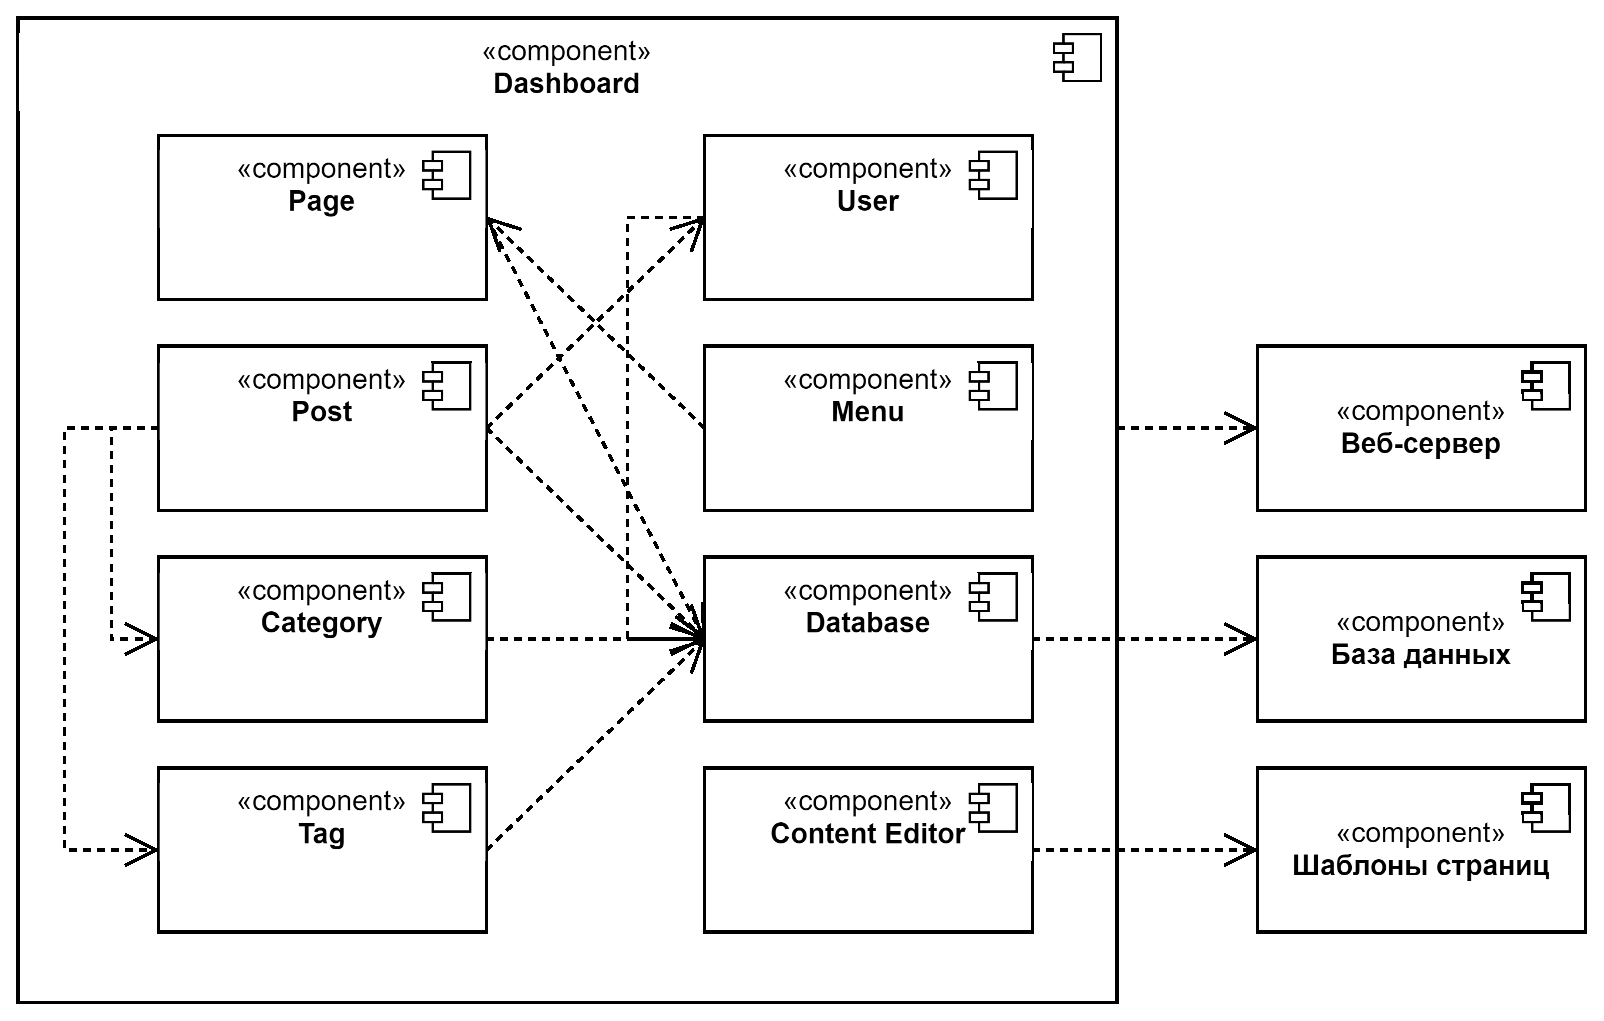
\includegraphics[width=1\linewidth]{comp}}
	\caption{Диаграмма компонентов}
	\label{comp:image}
\end{figure}

Описание компонентов программной системы:
\begin{enumerate}
	\item Page -- отвечает за создание и управление статическими страницами и организацию разделов сайта.
	\item Post -- используется для управления динамическим контентом, таким как статьи в блоге, новости, обновления и другие материалы, которые публикуются регулярно.
	\item Category -- используется для организации контента на сайте, содержит функции для структурирования постов по темам или разделам.
	\item Tag -- используется для дополнительной классификации контента, предоставляет более гибкую систему организации, чем категории, позволяя распределять посты по ключевым словам или темам.
	\item User -- этот компонент управляет информацией о пользователях сайта. Включает создание, редактирование и удаление учетных записей, управление ролями и правами доступа.
	\item Menu -- обеспечивает навигацию по сайту. Этот компонент позволяет создавать и управлять навигационными меню, которые могут содержать ссылки на страницы, посты, категории и другие элементы сайта.
	\item Content Editor -- представляет инструмент для создания и редактирования текстового и мультимедийного контента на сайте. Обычно он включает в себя визуальный интерфейс который позволяет пользователям форматировать текст, вставлять изображения, видео, ссылки и другие элементы без необходимости писать HTML код.
	\item Database -- обеспечивает создание и управление данными которые храняться в таблицах БД, отвечает за выполнение запросов к базе данных для получения, добавления, обновления и удаления информации.
\end{enumerate}

\subsubsection{Классы программной системы}
На рисунке \ref{ui1:image} представлена диаграмма классов программной системы.

\begin{figure}[ht]
	\center{
\includegraphics[width=1\linewidth]{class}}
	\caption{Диаграмма классов}
	\label{class:image}
\end{figure}

\subsection{Проектирование пользовательского интерфейса программной системы}

На основании требований к пользовательскому интерфейсу представленных в пункте \ref{interface_requirements} технического задания, был разработан интерфейс администранивной панели системы и интерфейс редактора контента. Для создания пользовательского интерфейса используется язык разметки HTML и веб-фреймворк Bootstrap 5.

На рисунке \ref{ui1:image} представлен макет главного окна однистративной панели CMS. Макет содержит следующие элементы:
\begin{enumerate}
	\item Навигационное меню для перехода в соответствующий раздел панели управления.
	\item Область отображения содержимого текущего раздела.
\end{enumerate}
\begin{figure}[ht]
	\center{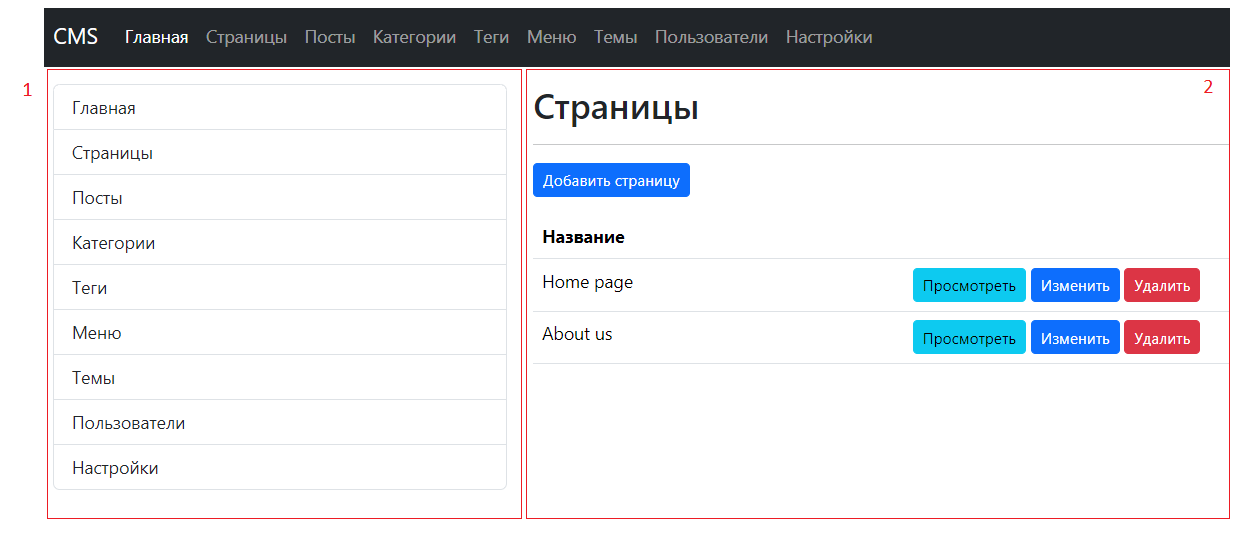
\includegraphics[width=1\linewidth]{ui1}}
	\caption{Макет главного окна панели управления}
	\label{ui1:image}
\end{figure}
На рисунке \ref{ui2:image} представлен макет раздела управления страницами. Макет содержит следующие элементы:
\begin{enumerate}
	\item Кнопку "<Добавить страницу"> для добавленя новой страницы.
	\item Список страниц сайта.
	\item Название соответствующей страницы.
	\item Кнопки управления страницей.
\end{enumerate}
\begin{figure}[ht]
	\center{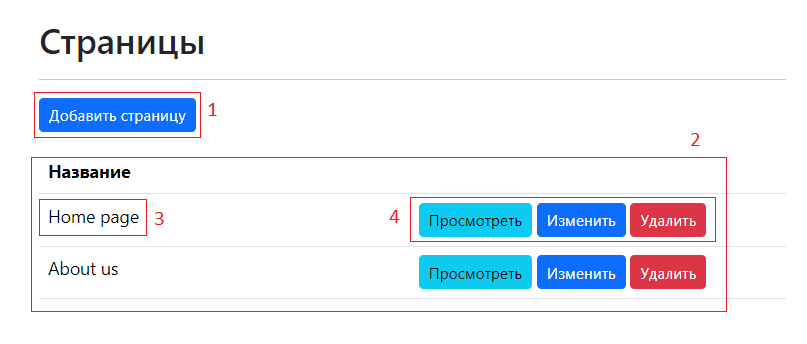
\includegraphics[width=1\linewidth]{ui2}}
	\caption{Макет раздела управления страницами}
	\label{ui2:image}
\end{figure}
На рисунке \ref{ui3:image} представлен макет раздела управления областями меню. Макет содержит следующие элементы:
\begin{enumerate}
	\item Список областей меню сайта.
	\item Кнопку "<Изменить"> для перехода на страницу управления пунктами выбранной области меню.
\end{enumerate}
\begin{figure}[ht]
	\center{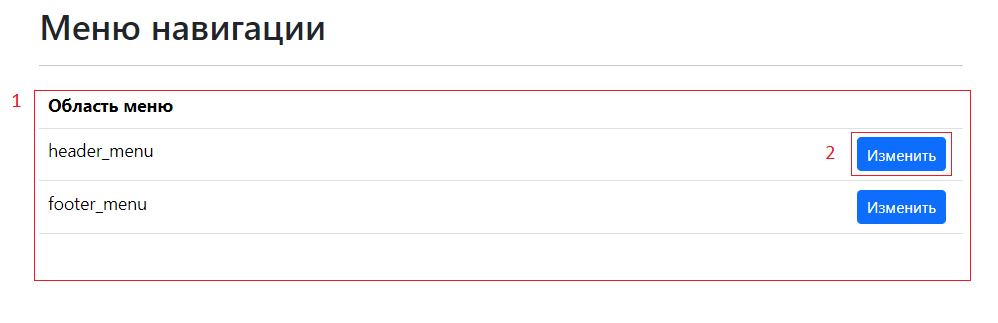
\includegraphics[width=1\linewidth]{ui3}}
	\caption{Макет раздела управления областями меню}
	\label{ui3:image}
\end{figure}
На рисунке \ref{ui4:image} представлен макет раздела управления пунктами меню. Макет содержит следующие элементы:
\begin{enumerate}
	\item Кнопку "<Добавить"> для добавленя нового пункта меню.
	\item Список пунктов меню.
	\item Кнопку для просмотра дочерних пунктов меню.
\end{enumerate}
\begin{figure}[ht]
	\center{
\includegraphics[width=1\linewidth]{ui4}}
	\caption{Макет раздела управления пунктами меню}
	\label{ui4:image}
\end{figure}
\ifПрактика{}\else{
   \section{Рабочий проект}
\subsection{Классы, используемые при разработке сайта}

Можно выделить следующий список классов и их методов, использованных при разработке web-приложения (таблица \ref{class:table}). Пример таблицы с уменьшенным межстрочным интервалом.

\renewcommand{\arraystretch}{0.8} % уменьшение расстояний до сетки таблицы
\begin{xltabular}{\textwidth}{|X|p{2.5cm}|>{\setlength{\baselineskip}{0.7\baselineskip}}p{4.85cm}|>{\setlength{\baselineskip}{0.7\baselineskip}}p{4.85cm}|}
\caption{Описание классов Bitrix, используемых в приложении\label{class:table}}\\
\hline \centrow \setlength{\baselineskip}{0.7\baselineskip} Название класса & \centrow \setlength{\baselineskip}{0.7\baselineskip} Модуль, к которому относится класс & \centrow Описание класса & \centrow Методы \\
\hline \centrow 1 & \centrow 2 & \centrow 3 & \centrow 4\\ \hline
\endfirsthead
\caption*{Продолжение таблицы \ref{class:table}}\\
\hline \centrow 1 & \centrow 2 & \centrow 3 & \centrow 4\\ \hline
\finishhead
CMain & Главный модуль & CMain – главный класс страницы web-приложения. После одного из этапов по загрузке страницы в сценарии становится доступным инициализированный системой объект данного класса с именем \$APPLICATION & void ShowTitle(string property\_code = «title», bool strip\_tags = true)
Выводит заголовок страницы
void SetTitle(string title)
Устанавливает заголовок страницы

void ShowCSS(bool external = true, bool XhtmlStyle = true)
Выводит таблицу стилей CSS страницы\\
\hline CFile & Главный модуль & CFile – Класс для работы с файлами и изображениями & array GetFileArray (int file\_id)
Метод возвращает массив, содержащий описание файла (путь к файлу, имя файла, размер) с идентификатором file\_id
\end{xltabular}
\renewcommand{\arraystretch}{1.0} % восстановление сетки

\subsection{Модульное тестирование разработанного web-сайта}

Модульный тест для класса User из модели данных представлен на рисунке \ref{unitUser:image}.

\begin{figure}[ht]
\begin{lstlisting}[language=Python]
from django.test import TestCase
from .models import *
User = get_user_model()


class ShpoTestCases(TestCase):

    def setUp(self) -> None:
        self.user = User.objects.create(username='testtestovich', password='testtestovich', first_name='Sad', last_name='')

    def test_2(self):

        self.assertEqual(self.user.first_name, 'Sad')
        self.assertEqual(self.user.last_name, 'Cat')
        print((self.user))
        print((self.user.first_name))
        print((self.user.last_name))
\end{lstlisting}  
\caption{Модульный тест класса User}
\label{unitUser:image}
\end{figure}

\subsection{Системное тестирование разработанного web-сайта}

На рисунке \ref{main:image} представлена главная страница сайта «Русатом – Аддитивные технологии».
\newpage % при необходимости можно переносить рисунок на новую страницу
\begin{figure}[H] % H - рисунок обязательно здесь, или переносится, оставляя пустоту
\center{\includegraphics[width=1\linewidth]{main1}}
\center{\includegraphics[width=1\linewidth]{main2}}
\center{\includegraphics[width=1\linewidth]{main3}}
\caption{Главная страница сайта «Русатом – Аддитивные технологии»}
\label{main:image}
\end{figure}

На рисунке \ref{menu:image} представлен динамический вывод заголовков, включающий в себя искомые фразы при поиске фраз.

\begin{figure}[ht]
\center{\includegraphics[width=1\linewidth]{menu}}
\caption{Динамический вывод заголовков}
\label{menu:image}
\end{figure}

На рисунке \ref{enter:image} представлен ввод данных для публикации новости.

\begin{figure}[ht]
\center{\includegraphics[width=1\linewidth]{enter}}
\caption{Ввод данных для публикации очень-очень длинной, интересной и полезной новости}
\label{enter:image}
\end{figure}

   \section*{ЗАКЛЮЧЕНИЕ}
\addcontentsline{toc}{section}{ЗАКЛЮЧЕНИЕ}

Преимущества аддитивных технологий заключается в разнообразии процессов, позволяющих применять их в различных областях производства. Существенным ограничением же является и экономическая составляющая, которая не позволит внедрить аддитивное производство повсеместно.
  
Компании, видя, как развиваются информационные технологии, пытаются использовать их выгодно для своего бизнеса, запуская свой сайт для того, чтобы заявить о своем существовании, проинформировать потенциального клиента об услугах или продуктах, которые предоставляет. 
Для продвижения компании «Русатом – Аддитивные технологии» был разработан веб-сайт на основе системы «1С-Битрикс: Управление сайтом».

Основные результаты работы:

\begin{enumerate}
\item Проведен анализ предметной области. Выявлена необходимость использовать 1С-Битрикс.
\item Разработана концептуальная модель web-сайта. Разработана модель данных системы. Определены требования к системе.
\item Осуществлено проектирование web-сайта. Разработана архитектура серверной части. Разработан пользовательский интерфейс web-сайта.
\item Реализован и протестирован web-сайт. Проведено модульное и системное тестирование.
\end{enumerate}

Все требования, объявленные в техническом задании, были полностью реализованы, все задачи, поставленные в начале разработки проекта, были также решены.

Готовый рабочий проект представлен адаптивной версткой сайта. Сайт находится в публичном доступе, поскольку опубликован в сети Интернет.  

}\fi
\addcontentsline{toc}{section}{СПИСОК ИСПОЛЬЗОВАННЫХ ИСТОЧНИКОВ}

\begin{thebibliography}{9}

    \bibitem{javascript} Фримен, А. Практикум по программированию на JavaScript / А. Фримен. – Москва~: Вильямс, 2013. – 960 с. – ISBN 978-5-8459-1799-7. – Текст~: непосредственный.
    \bibitem{php} Бретт, М. PHP и MySQL. Исчерпывающее руководство / М. Бретт. – Санкт-Петербург : Питер, 2016. – 544 с. – ISBN 978-5-496-01049-8. – Текст~: непосредственный.
    \bibitem{css} Веру, Л. Секреты CSS. Идеальные решения ежедневных задач / Л. Веру. – Санкт-Петербург : Питер, 2016. – 336 с. – ISBN 978-5-496-02082-4. – Текст~: непосредственный.
    \bibitem{mysql}	Гизберт, Д. PHP и MySQL / Д. Гизберт. – Москва~: НТ Пресс, 2013. – 320 с. – ISBN 978-5-477-01174-2. – Текст~: непосредственный.
	\bibitem{html5}	Голдстайн, А. HTML5 и CSS3 для всех / А. Голдстайн, Л. Лазарис, Э. Уэйл. – Москва~: Вильямс, 2012. – 368 с. – ISBN 978-5-699-57580-0. – Текст~: непосредственный.
	\bibitem{htmlcss}	Дэкетт, Д. HTML и CSS. Разработка и создание веб-сайтов / Д. Дэкетт. – Москва~: Эксмо, 2014. – 480 с. – ISBN 978-5-699-64193-2. – Текст~: непосредственный.
	\bibitem{bigbook}	Макфарланд, Д. Большая книга CSS / Д. Макфарланд. – Санкт-Петербург : Питер, 2012. – 560 с. – ISBN 978-5-496-02080-0. – Текст~: непосредственный.
	\bibitem{uchiru}	Лоусон, Б. Изучаем HTML5. Библиотека специалиста / Б. Лоусон, Р. Шарп. – Санкт-Петербург : Питер, 2013 – 286 с. – ISBN 978-5-459-01156-2. – Текст~: непосредственный.
	\bibitem{chaynik}	Титтел, Э. HTML5 и CSS3 для чайников / Э. Титтел, К. Минник. – Москва~: Вильямс, 2016 – 400 с. – ISBN 978-1-118-65720-1. – Текст~: непосредственный.    
	\bibitem{22}	Титтел, Э. HTML5 и CSS3 для чайников / Э. Титтел, К. Минник. – Москва~: Вильямс, 2016 – 400 с. – ISBN 978-1-118-65720-1. – Текст~: непосредственный.    
	\bibitem{1231}	Титтел, Э. HTML5 и CSS3 для чайников / Э. Титтел, К. Минник. – Москва~: Вильямс, 2016 – 400 с. – ISBN 978-1-118-65720-1. – Текст~: непосредственный.    
	\bibitem{sdf}	Титтел, Э. HTML5 и CSS3 для чайников / Э. Титтел, К. Минник. – Москва~: Вильямс, 2016 – 400 с. – ISBN 978-1-118-65720-1. – Текст~: непосредственный.    
	\bibitem{servsssds}	Титтел, Э. HTML5 и CSS3 для чайников / Э. Титтел, К. Минник. – Москва~: Вильямс, 2016 – 400 с. – ISBN 978-1-118-65720-1. – Текст~: непосредственный.
\end{thebibliography}

\ifВКР{\appendix{Представление графического материала}

Графический материал, выполненный на отдельных листах,
изображен на рисунках А.1--А.\arabic{числоПлакатов}.
\setcounter{числоПлакатов}{0}

\renewcommand{\thefigure}{А.\arabic{figure}} % шаблон номера для плакатов

\begin{landscape}

\begin{плакат}
    
\includegraphics[width=0.82\linewidth]{плакат1.png}
    \заголовок{Сведения о ВКРБ}
    \label{pl1:image}      
\end{плакат}

\begin{плакат}
    
\includegraphics[width=0.82\linewidth]{плакат2.png}
    \заголовок{Цель и задачи разработки}
    \label{pl2:image}      
\end{плакат}

\begin{плакат}
    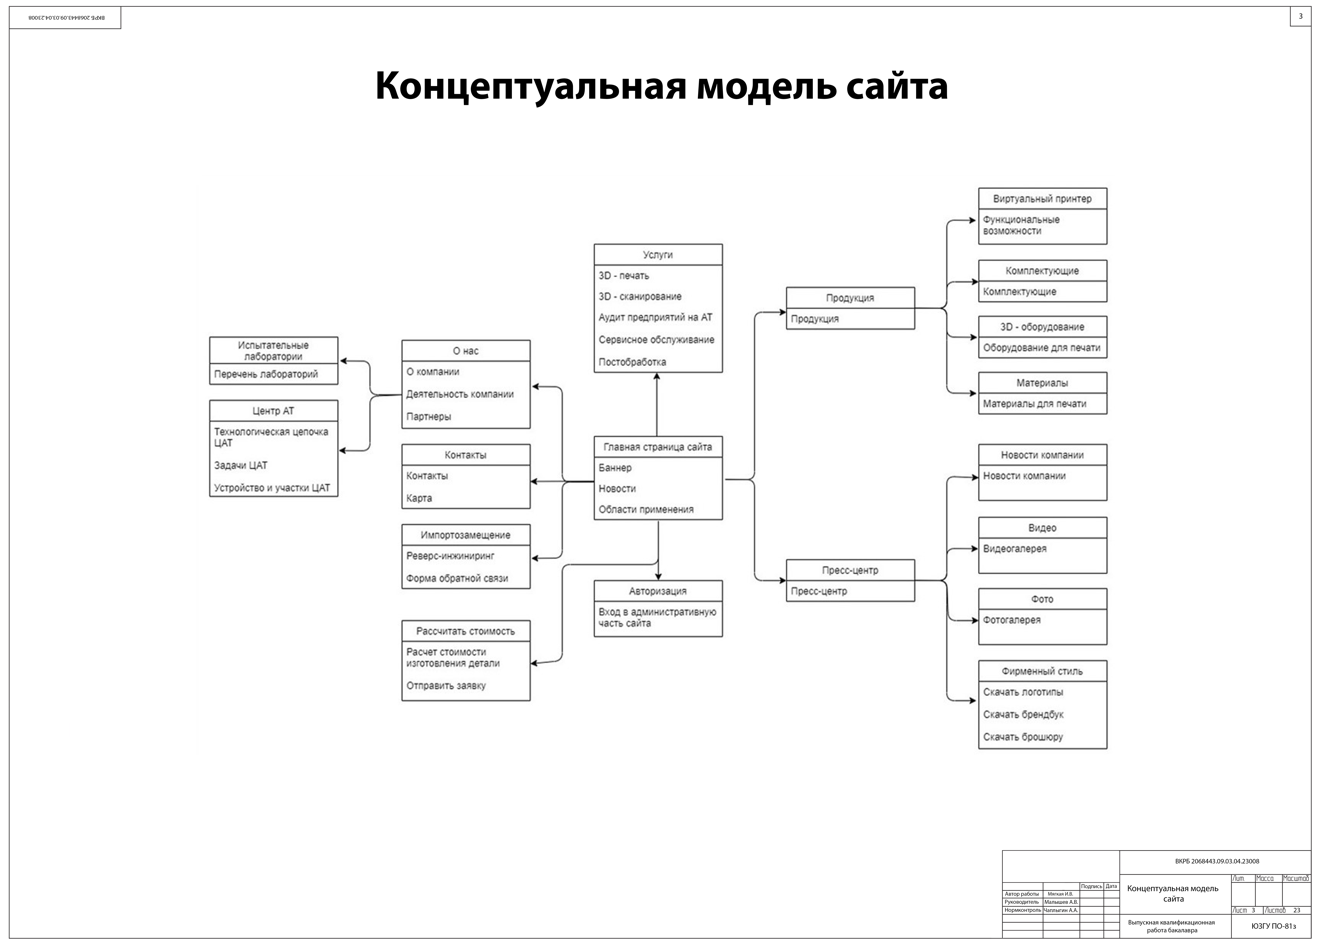
\includegraphics[width=0.82\linewidth]{плакат3.png}
    \заголовок{Концептуальная модель сайта}
    \label{pl3:image}      
\end{плакат}

\begin{плакат}
    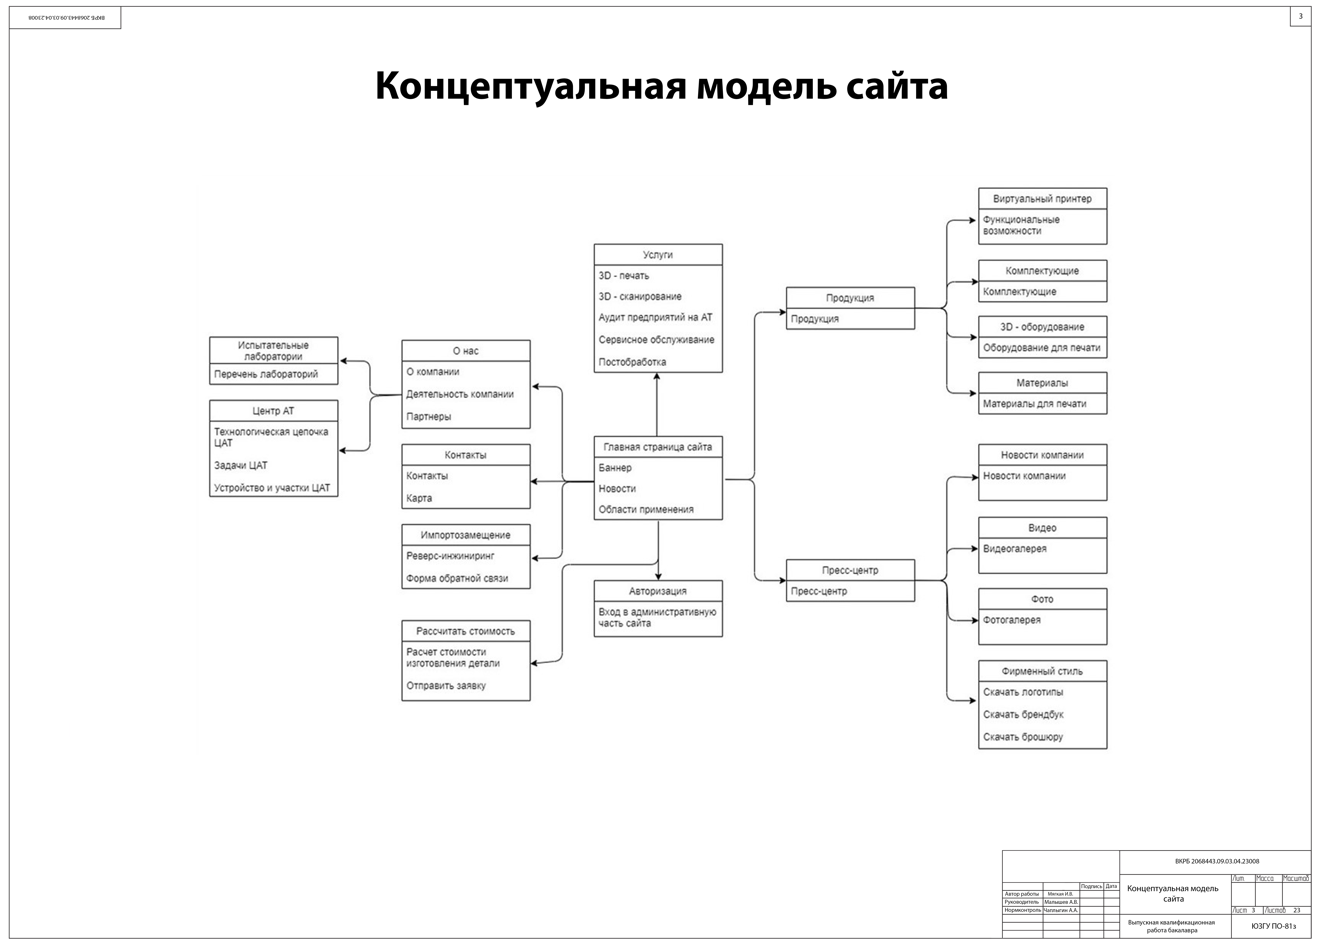
\includegraphics[width=0.82\linewidth]{плакат3.png}
    \заголовок{Еще плакат}
    \label{pl4:image}      
\end{плакат}

\end{landscape}
}\fi
\ifПрактика{}\else{\appendix{Фрагменты исходного кода программы}

main.tex
\lstinputlisting[language=Tex, frame=none]{main.tex}

ТехПроект.tex
\lstinputlisting[language=Tex, frame=none]{ТехПроект.tex}

\ifВКР{
\newpage
\addcontentsline{toc}{section}{На отдельных листах (CD-RW в прикрепленном конверте)}
\begin{center}
\textbf{Место для диска}
\end{center}
}\fi
}\fi
\end{document}
